% !TEX encoding = UTF-8 Unicode
\documentclass{article}

\usepackage{polski}
\usepackage[utf8]{inputenc}
\usepackage{subfig}
\usepackage{multirow}
\usepackage{graphicx}

\usepackage[a4paper, left=2.5cm, right=2.5cm, top=3.5cm, bottom=3.5cm, headsep=1.2cm]{geometry}

\linespread{1.3}
\begin{document}
	
	\begin{titlepage}
		\centering
		{\scshape\LARGE Politechnika Wrocławska \par}
		{\scshape\Large Katedra Informatyki Technicznej\par}
		
		\vspace{1cm}
		{\scshape\Large Inżynieria Oprogramowania\par}
		\vspace{1.5cm}
		{\huge\bfseries \par}
		\vspace{2cm}
		{\Large\itshape Magdalena Biernat\par}
		{\Large\itshape Mateusz Bortkiewicz\par}
		\vfill
		Opiekun\par
		prof. dr hab. inż. Jan Magott 
		
		\vfill
		{\large \today\par}
	\end{titlepage}
	\newpage
	\section{Wprowadzenie}
	Sprawozdanie dotyczy jedenastych zajęć. Na tych laboratoriach kontynuowaliśmy swój projekt. 
	
	\subsection{Cel laboratorium}
	Opracowanie diagramu stanów dla wybranej klasy, reprezentującego wpływ różnych przypadków użycia na	zmiany stanów tej klasy, modelowanych za pomocą	diagramów sekwencji.
	\subsection{Diagram stanów kalkulatora}
	\begin{figure}[!ht]
		\centering
		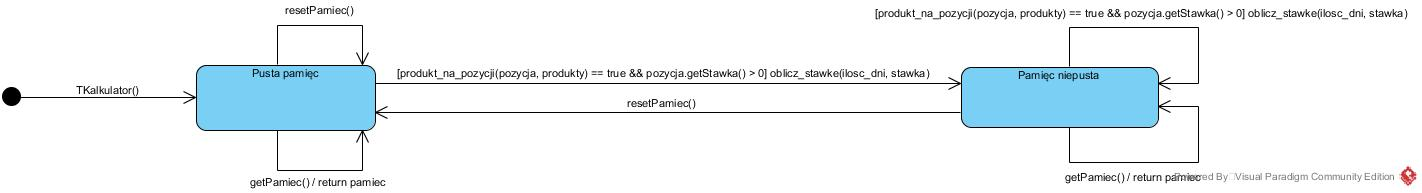
\includegraphics[width=18cm]{1.jpg}
		\caption{Stworzony diagram stanów}
		\label{fig:obrazek 1}
		\newpage
	\end{figure}
	\subsection{Diagram stanów metody szukaj\_TWypozyczenia}
	\begin{figure}[!ht]
		\centering
		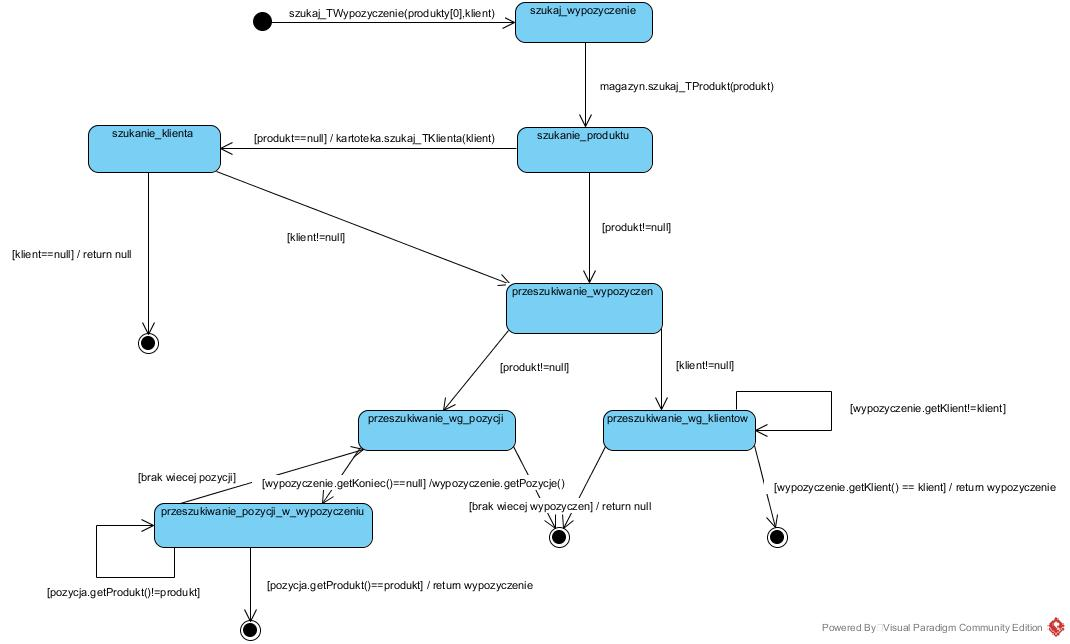
\includegraphics[width=18cm]{2.jpg}
		\caption{Stworzony diagram stanów}
		\label{fig:obrazek 2}
		\newpage
	\end{figure}
\subsection{Kod}
Zostały również naniesione pojedyncze zmiany w kodzie
\end{document}